% !TeX spellcheck = it_IT
\newpage
\section{Concorrenza}
Il sistema operativo deve gestire molte cose contemporaneamente (\textbf{MTAO} - Multiple Things at Once): processi, interrupts, manutenzione di background, etc...
Non è solo il SO che deve gestire tutti questi aspetti, ma anche \emph{server} (garantire più connessioni simultanee), \emph{programmi} (migliori performance), \emph{interfacce} (aumentare la responsiveness), \emph{network} e \emph{dischi} (ridurre la latenza).

\begin{note}
	Il parallelismo è quando del codice può essere eseguito effettivamente nello stesso momento mentre la concorrenza è più virtuale: è lo scheduler che alterna i processi.
\end{note}

\subsection{Inter-Process Communication}
La concorrenza porta i processi ad avere un loro spazio di memoria riservato e si rende quindi necessario un \textbf{Inter-Process Communication} (IPC) per scambiare le informazioni e sincronizzarsi. C'è quindi un maggiore \emph{overhead} di comunicazione.
\begin{center}
	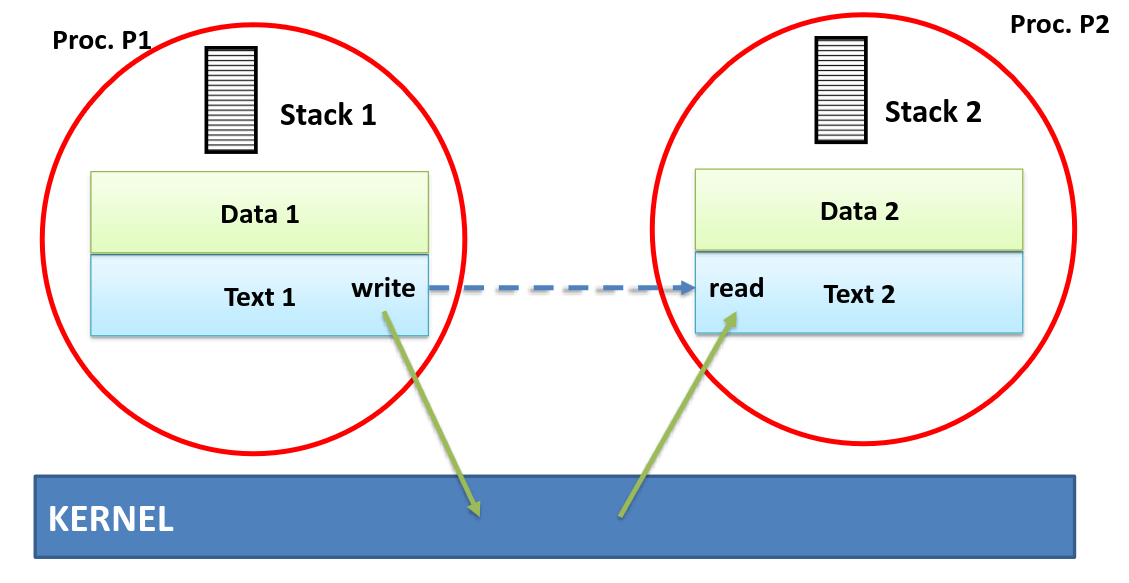
\includegraphics[scale=0.3]{ipc.png}
\end{center}


\subsection{Thread}
I thread sono singole entità che eseguono una \textbf{task indipendente} (può essere messa in pausa del SO). Condividono la memoria del processo che li crea, poiché fanno parte dello stesso spazio di memoria, ed eseguono un pezzo di codice. \\
Il vantaggio principale è il fatto che non si deve più passare dal SO per comunicare e c'è quindi un vantaggio \textbf{prestazionale}. Inoltre migliora l'\textbf{organizzazione} della struttura codice.

\subsubsection{Protezione}
Rimane che il thread può accedere solamente alla memoria del suo processo, garantendo così la protezione. C'è però da prestare attenzione ad evitare che un thread acceda ai dati di un altro thread nello stesso processo. In questo caso si SO non rileva errori.

\subsubsection{Astrazione}
Ogni processo può creare virtualmente infiniti thread. Lo sviluppatore non sa in che ordine e con che velocità verrà poi eseguito ognuno di essi, dato che viene gestito dal kernel, e deve quindi progettare il software in modo che possa funzionare indipendentemente dalla schedule.
\begin{center}
	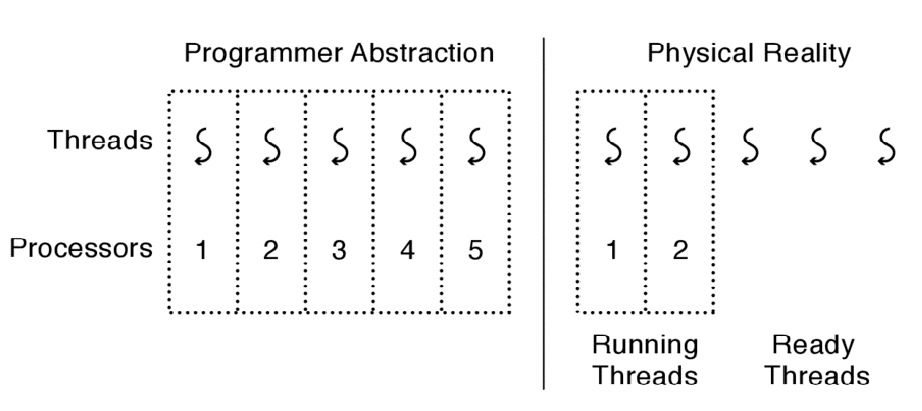
\includegraphics[scale=0.2]{thread_abstraction.png}
\end{center}

\subsubsection{Implementazione}
Alla base dei thread troviamo il \textbf{Thread Control Block} (TCB), ovvero una struttura dati che contiene le informazioni necessarie al thread. È necessario inoltre definire \textbf{operazioni} sui thread e uno \textbf{scheduler}, ovvero una funzione del sistema operativo che si occupi di assegnargli dei processori.\\
Lo scheduler viene mandato in esecuzione periodicamente dal SO tramite degli interrupt attivati dal \textbf{timer}:
\begin{center}
	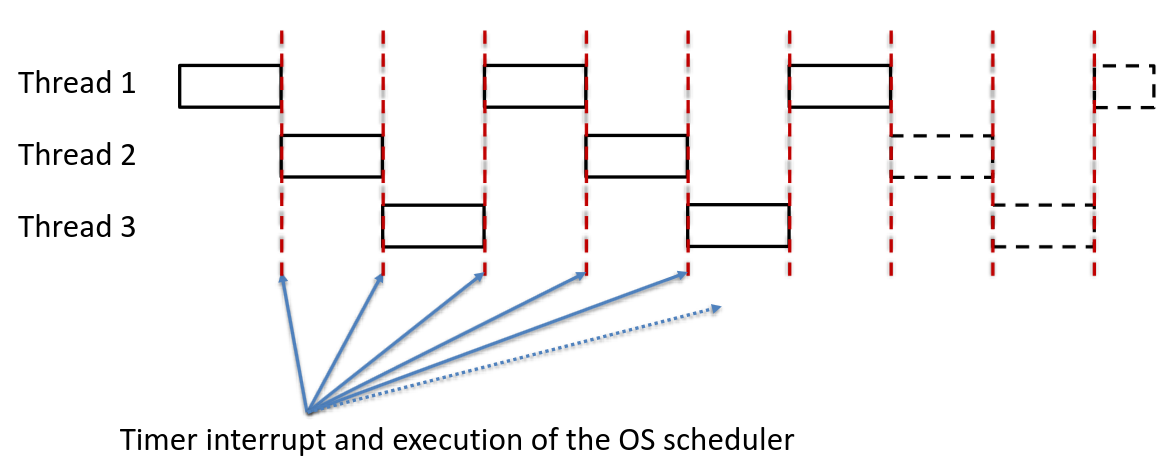
\includegraphics[scale=0.3]{thread_scheduler.png}
\end{center}
Distinguiamo due tipi di thread:
\begin{itemize}
	\item \textbf{Cooperative}: \label{thread_types}cooperano tra di loro in modo esplicito, ovvero con particolari istruzioni viene controllato lo scheduler. Finché non viene dato un comando o finché non scade il timer, rimane attivo quel thread
	\item \textbf{Preemptive}: partono e possono essere fermati dal SO in qualunque momento
\end{itemize}
che possono essere implementati in modi diversi:
\begin{itemize}
	\item Processi multipli \textbf{single-threaded}
	\item Processi multipli all'interno di un singolo processo, dove lo scheduler è gestito da una libreria (\textbf{user-level threads})
	\item \textbf{Misto} tra single e multi-threaded (\textbf{kernel-level threads})
	\item \textbf{Scheduler activation}
\end{itemize}

\subsubsection{API}
\begin{itemize}
	\item \textbf{create(thread, func, args)}: crea un thread e lo salva in \emph{thread}, poi esegue \emph{func} con gli argomenti in \emph{args}
	\item \textbf{yield()}: il thread smette volontariamente di usare il processore per dare spazio ad altri
	\item \textbf{join(thread)}: attende che il \emph{thread} finisca e a quel punto restituisce lo stato di uscita
	\item \textbf{exit(status)}: termina il thread corrente con un determinato \emph{status} 
\end{itemize}

\subsubsection{Ciclo di vita}
\begin{center}
	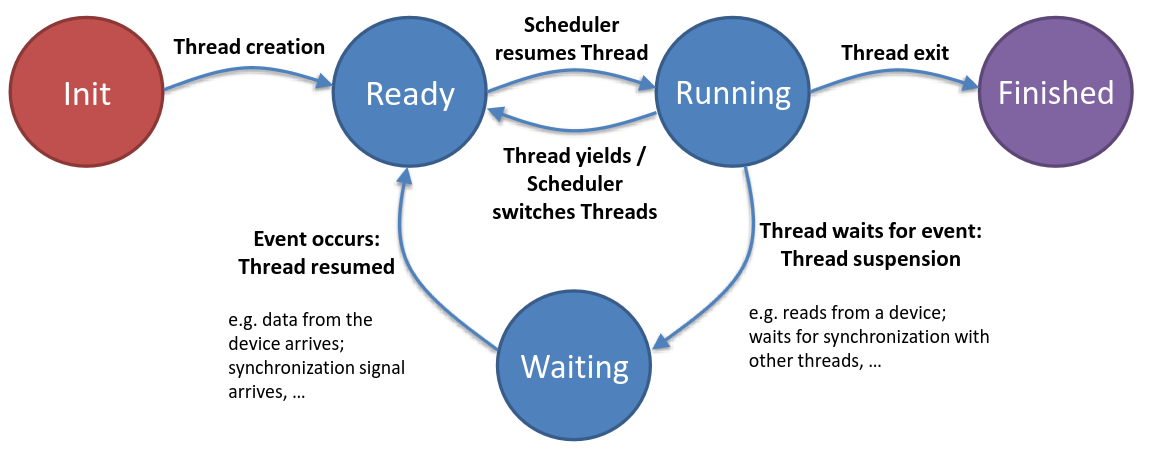
\includegraphics[scale=0.37]{thread_lifecycle.png}
\end{center}
Tutti questi stati sono implementati tramite \textbf{code} (liste). Ogni stato ha diverse code.\\

Nella seguente tabella è indicato dove si trovano i registri in ogni stato del ciclo di vita. Riassumendo, l'unico caso in cui i registri non sono quelli del TCB, è quando il thread è in esecuzione, poiché in quel momento i registri validi sono nel processore.
\begin{center}
	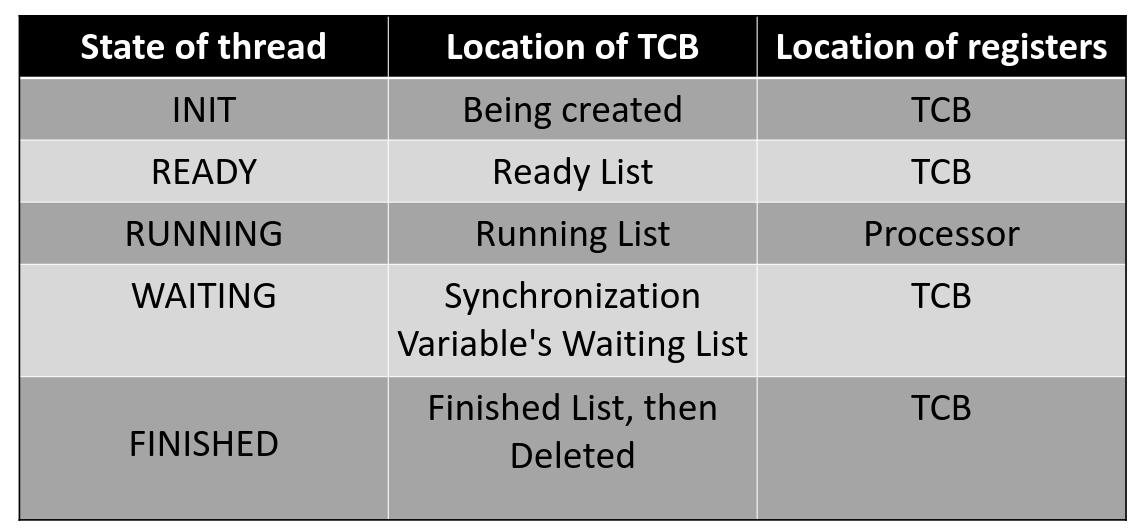
\includegraphics[scale=0.3]{tcb_register.png}
\end{center}

\subsubsection{User-level thread}
Sono implementati a livello utente, ovvero che il SO non è a conoscenza del fatto che un determinato processo sia al suo interno formato da più thread logici. Lo scheduling è quindi fatto da una libreria a livello utente: il \textbf{Run Time Support} (RTS).\\
Il modello utilizzato in questo schema è quello \textbf{cooperativo} (vedi \ref{thread_types}). Potrebbe essere implementato anche con il modello \textbf{preemptive} utilizzando le \emph{Scheduler Activation} di Windows o le \emph{UpCall}.\\
Il problema principale è che quando invoco una \textbf{system-call bloccante}, viene bloccato l'intero processo, dato che il SO non sa cosa c'è dentro al processo. Inoltre questa mancanza di conoscenza da parte del SO mi impedisce di sfruttare a pieno le risorse del sistema.